\documentclass[]{article}
\usepackage{lmodern}
\usepackage{amssymb,amsmath}
\usepackage{ifxetex,ifluatex}
\usepackage{fixltx2e} % provides \textsubscript
\ifnum 0\ifxetex 1\fi\ifluatex 1\fi=0 % if pdftex
  \usepackage[T1]{fontenc}
  \usepackage[utf8]{inputenc}
\else % if luatex or xelatex
  \ifxetex
    \usepackage{mathspec}
  \else
    \usepackage{fontspec}
  \fi
  \defaultfontfeatures{Ligatures=TeX,Scale=MatchLowercase}
\fi
% use upquote if available, for straight quotes in verbatim environments
\IfFileExists{upquote.sty}{\usepackage{upquote}}{}
% use microtype if available
\IfFileExists{microtype.sty}{%
\usepackage{microtype}
\UseMicrotypeSet[protrusion]{basicmath} % disable protrusion for tt fonts
}{}
\usepackage[margin=1in]{geometry}
\usepackage{hyperref}
\hypersetup{unicode=true,
            pdftitle={Simulation summary},
            pdfauthor={Xuelong Wang},
            pdfborder={0 0 0},
            breaklinks=true}
\urlstyle{same}  % don't use monospace font for urls
\usepackage{graphicx,grffile}
\makeatletter
\def\maxwidth{\ifdim\Gin@nat@width>\linewidth\linewidth\else\Gin@nat@width\fi}
\def\maxheight{\ifdim\Gin@nat@height>\textheight\textheight\else\Gin@nat@height\fi}
\makeatother
% Scale images if necessary, so that they will not overflow the page
% margins by default, and it is still possible to overwrite the defaults
% using explicit options in \includegraphics[width, height, ...]{}
\setkeys{Gin}{width=\maxwidth,height=\maxheight,keepaspectratio}
\IfFileExists{parskip.sty}{%
\usepackage{parskip}
}{% else
\setlength{\parindent}{0pt}
\setlength{\parskip}{6pt plus 2pt minus 1pt}
}
\setlength{\emergencystretch}{3em}  % prevent overfull lines
\providecommand{\tightlist}{%
  \setlength{\itemsep}{0pt}\setlength{\parskip}{0pt}}
\setcounter{secnumdepth}{5}
% Redefines (sub)paragraphs to behave more like sections
\ifx\paragraph\undefined\else
\let\oldparagraph\paragraph
\renewcommand{\paragraph}[1]{\oldparagraph{#1}\mbox{}}
\fi
\ifx\subparagraph\undefined\else
\let\oldsubparagraph\subparagraph
\renewcommand{\subparagraph}[1]{\oldsubparagraph{#1}\mbox{}}
\fi

%%% Use protect on footnotes to avoid problems with footnotes in titles
\let\rmarkdownfootnote\footnote%
\def\footnote{\protect\rmarkdownfootnote}

%%% Change title format to be more compact
\usepackage{titling}

% Create subtitle command for use in maketitle
\newcommand{\subtitle}[1]{
  \posttitle{
    \begin{center}\large#1\end{center}
    }
}

\setlength{\droptitle}{-2em}

  \title{Simulation summary}
    \pretitle{\vspace{\droptitle}\centering\huge}
  \posttitle{\par}
    \author{Xuelong Wang}
    \preauthor{\centering\large\emph}
  \postauthor{\par}
      \predate{\centering\large\emph}
  \postdate{\par}
    \date{7/12/2018}

\usepackage{float}
\newcommand{\indep}{\rotatebox[origin=c]{90}{$\models$}}

\begin{document}
\maketitle

{
\setcounter{tocdepth}{2}
\tableofcontents
}
\section{Background of the environmental
study}\label{background-of-the-environmental-study}

The overall goal of this study is to find the relation between chemical
exposures and health outcome. Due to the complexity of the problem, we
have to tackle the problem step by step. More specifically, we want to
find a model to estimate the \textbf{cumulative(main)},
\textbf{interactive(interaction)}, and \textbf{separate} effects.

\section{Estimation of the Cumulative (main)
effect}\label{estimation-of-the-cumulative-main-effect}

Since the magnitudes of the covariates from the environmental study
(e.g.~PCB data) is small, the signal of the environmental factors will
probably be weak. This situation is very similar with what we got in the
\textbf{GWAS} study. Therefore, it's natural to pick up the approaches
used by GWAS studies. For example, the GCTA method.

\subsection{GCTA method}\label{gcta-method}

\subsubsection{Model}\label{model}

\[
  y_i = \beta_0 + \beta_{1}x_{i1}+\cdots+\beta_{m}x_{im} + \epsilon,    
\]

The matrix format is

\[
  Y = X\beta + \epsilon,    
\]

\begin{itemize}
\tightlist
\item
  If \(x's\) are standardized
\item
  and \(x_{ij} \indep x_{ij'}, \forall j \neq j'\)
\item
  and independent from \(\epsilon\), \[
    var(y) = var(\sum\beta_ix_i) + var(\epsilon) = \sum\beta^2_i + \sigma^2_{\epsilon} = \sigma^2_{\beta} + \sigma^2_{\epsilon}
  \] GCTA approach can estimate the \(\sigma^2_\beta\)
  \textbf{unbiaslly} without knowing the active causal set.
\end{itemize}

\subsection{\texorpdfstring{Proposed Method
(\textbf{uncorrelating})}{Proposed Method (uncorrelating)}}\label{proposed-method-uncorrelating}

To adopt GCTA approach, we need to transform the original data so that
they are independent to each other. The transformation is actually a
linear operation \(Z = XA^{-1}\). There one of task of this study is to
find an approparate matrix \(A\).

In the proposal, SVD method is used to find the \(A\). Although there is
some concern for that method, it seems that the correlation problem can
be solved well based on the simulation's result. There are high
correlation among the environmental data, but the proposed method can
estimate the main effect unbiaslly.

\subsubsection{Model}\label{model-1}

\[
  y_i = \alpha_0 + \alpha_{1}z_{i1}+\cdots+\alpha_{m}z_{im} + \epsilon,    
\]

The matrix format is

\[
  Y = Z\alpha + \epsilon,    
\] where \(Z = XA^{-1}\) and \(\alpha = A\beta\),

Then we have

\[
  var(Z\alpha) = var(X\beta)
\]

\section{Estimation of the interactive
effect}\label{estimation-of-the-interactive-effect}

In this case, we're not only interested in the main effect but also in
the interaction effect. It is possible that interaction effect also has
a contribution to the response. Besides, under the environmental study,
the total number of the covariates is much smaller than the GWAS study
so that considering the the interaction is also feasible.

\subsection{Model with interaction
terms}\label{model-with-interaction-terms}

\[
  y_i = \sum^m_{j = 1}x_j*\beta^{(main)}_j + \sum^{m(m-1)/2}_{j=1}x^{(inter)}_j\gamma^{(inter)}_j ~+~ \epsilon_i
\]

The variance of y could be decomposed as following:

\[
  var(y_i) = \sigma^2_{\beta} + \sigma^2_{\gamma} + \sigma^2_{\epsilon}
\]

\subsection{Issues of estimating the interaction
effect}\label{issues-of-estimating-the-interaction-effect}

If consider to use the GCTA approach, there is a large bias on the
estimation of the interaction effect. Based on the simulation results
from the proposal, the marginal distribution of the covariates may have
affected the proposed method's performance. It seems that it works well
under the normal distribution even give the correlation structure
between covariates.

\subsection{How does the covariate's distribution affect the
result?}\label{how-does-the-covariates-distribution-affect-the-result}

To check what influence of the normality will have on the performance, I
conduct several simulations studying which includes transforming and
selecting the covariates.

\subsubsection{Transformation}\label{transformation}

Since the data is right skewed, I consider log and square root
transformation. Besides, I also consider the rank and normal quantile
transformation. Categorized transformation is also used to improve the
normality

Based on the simulation results, Categorized transformation seems to
\textbf{reduce} the biasness of the proposed method when estimating
interaction

\subsubsection{simulation result}\label{simulation-result}

Basically, all the transformation methods improve the performance.
However, the bias issue is still not solved, especially for the proposed
method.

Following is the result of rank and normal quantile transformation. For
the graphs you can tell that the proposed method still has bias after
the transformation

\paragraph{Rank}\label{rank}

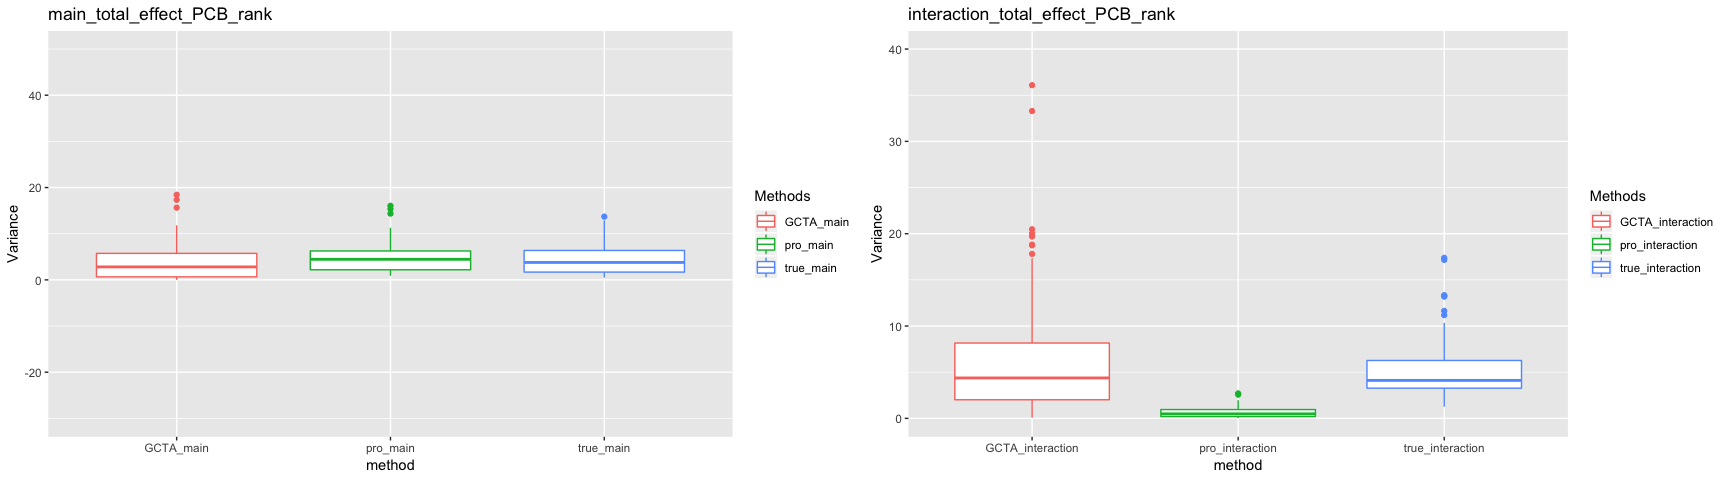
\includegraphics{./Transformation_simulation_files/figure-html/unnamed-chunk-15-1.png}
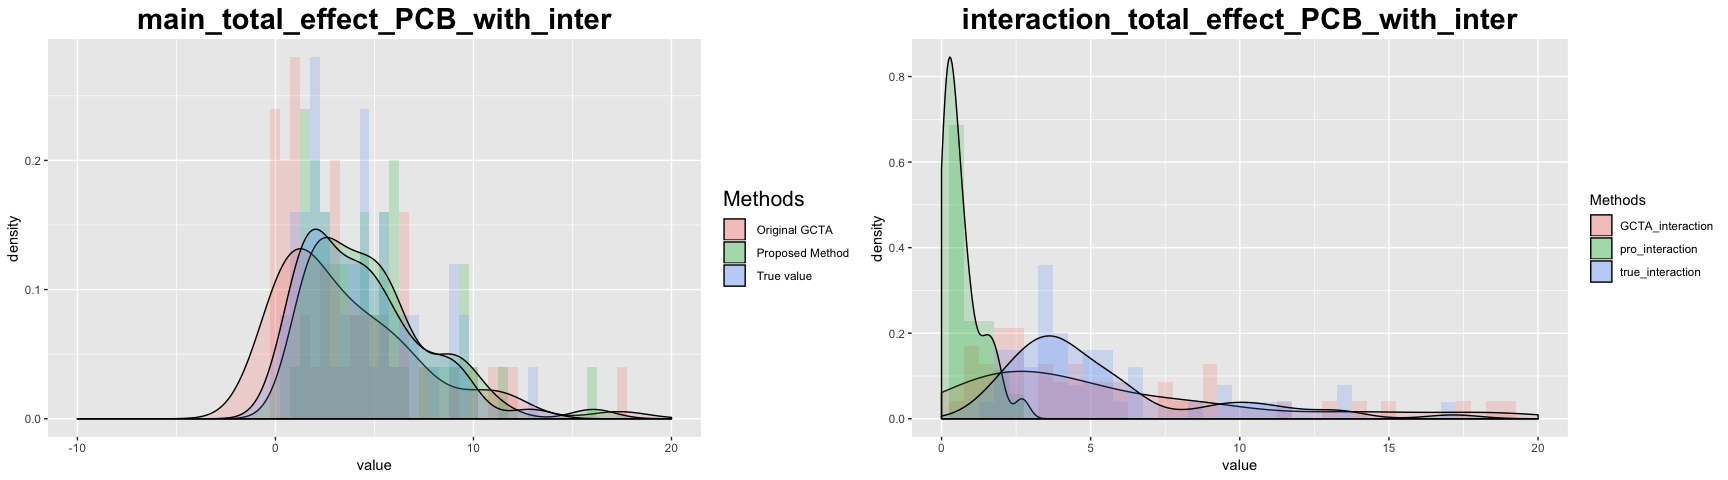
\includegraphics{./Transformation_simulation_files/figure-html/unnamed-chunk-16-1.png}

\paragraph{Normal quantile}\label{normal-quantile}

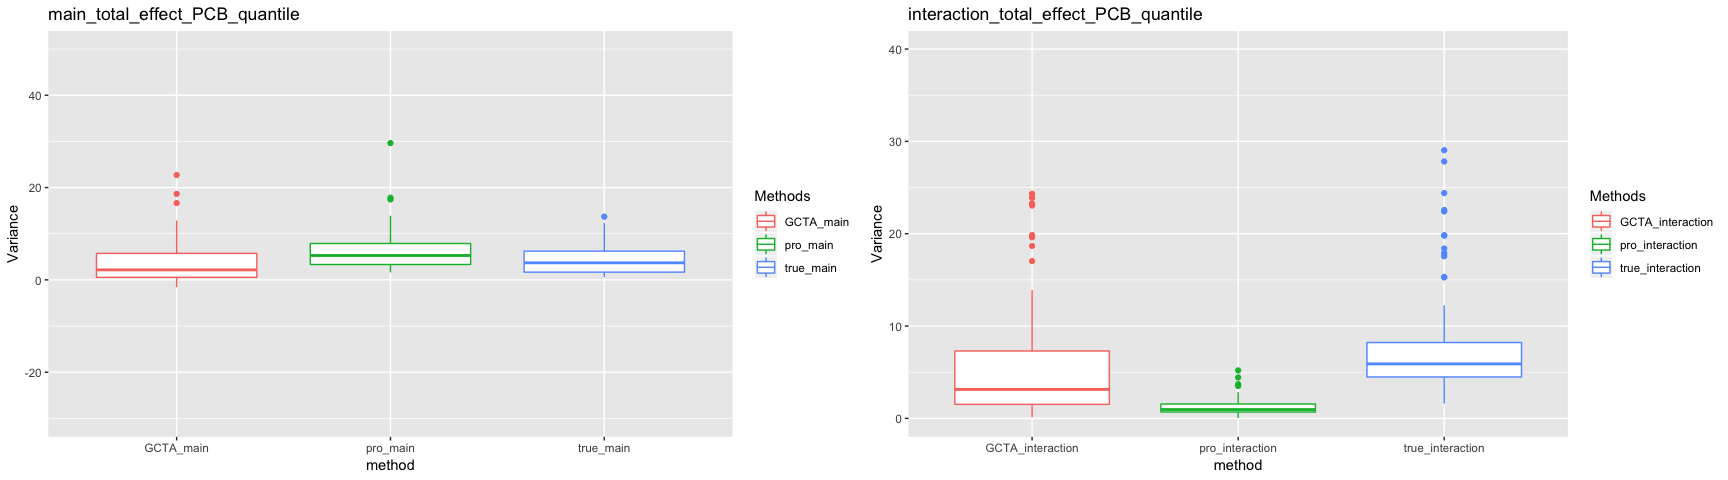
\includegraphics{./Transformation_simulation_files/figure-html/unnamed-chunk-18-1.png}
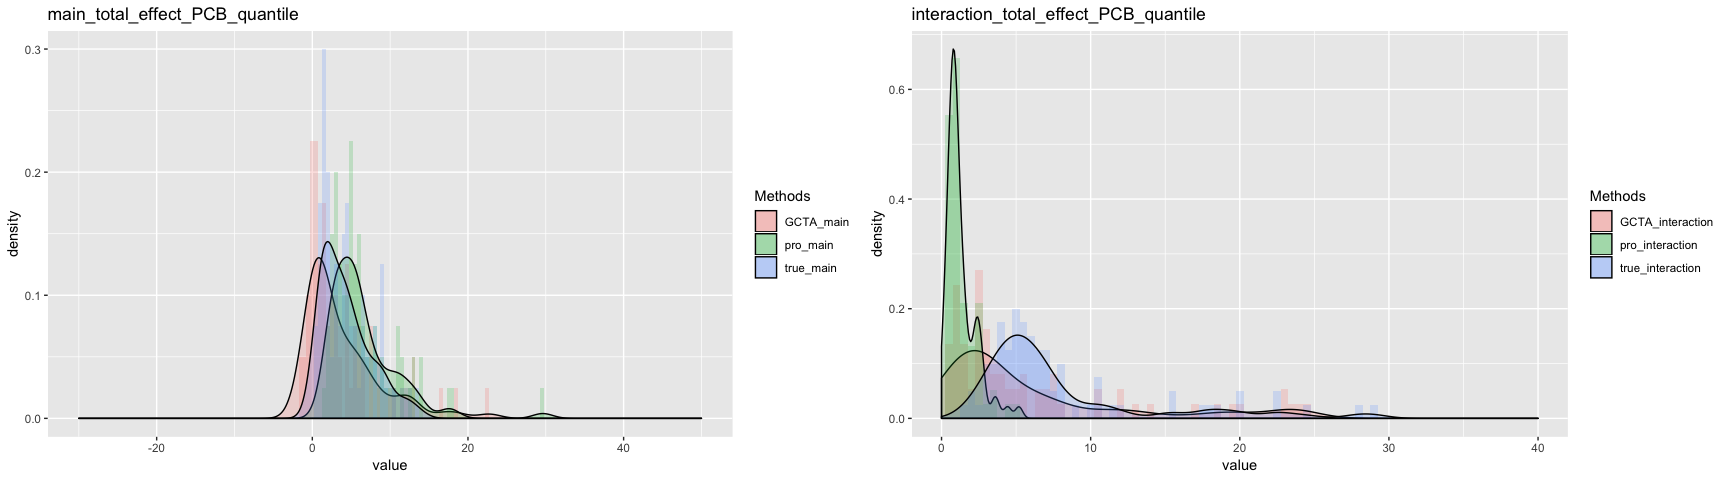
\includegraphics{./Transformation_simulation_files/figure-html/unnamed-chunk-19-1.png}

\paragraph{Categorized into 5 levels}\label{categorized-into-5-levels}

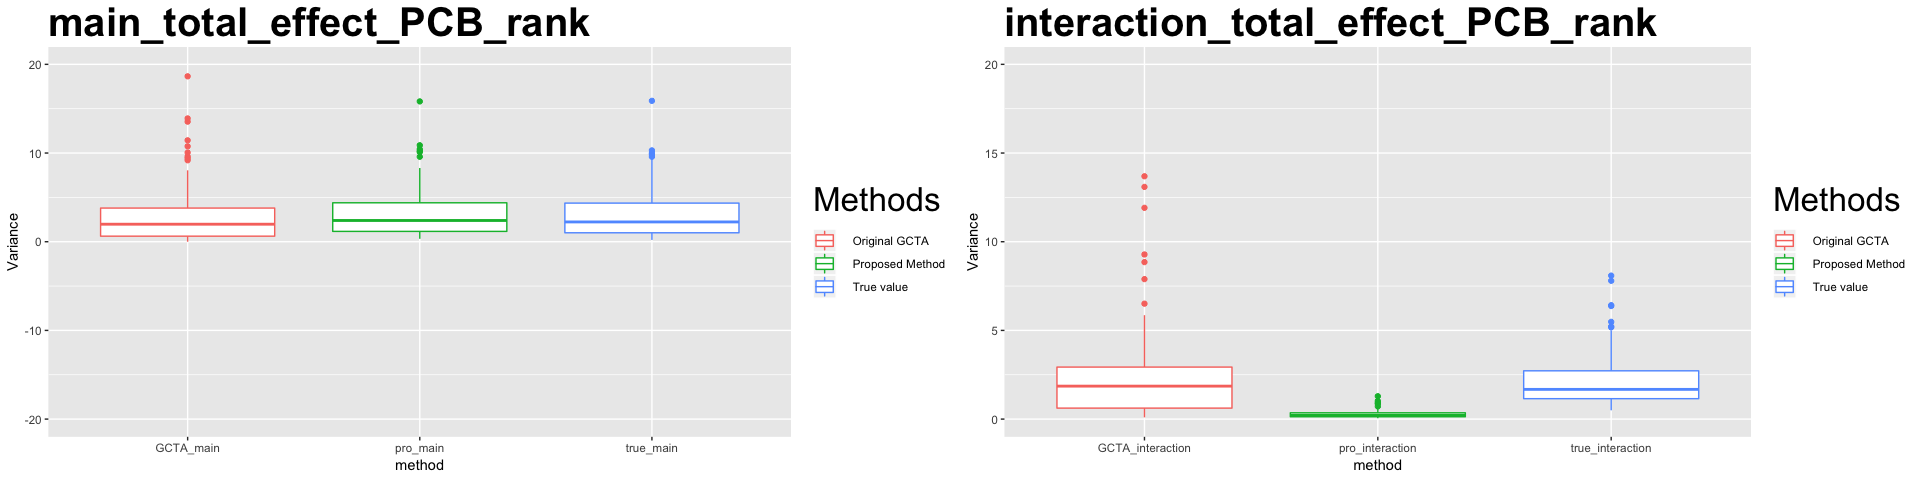
\includegraphics{./Categorize_simulation_files/figure-html/unnamed-chunk-5-1.png}
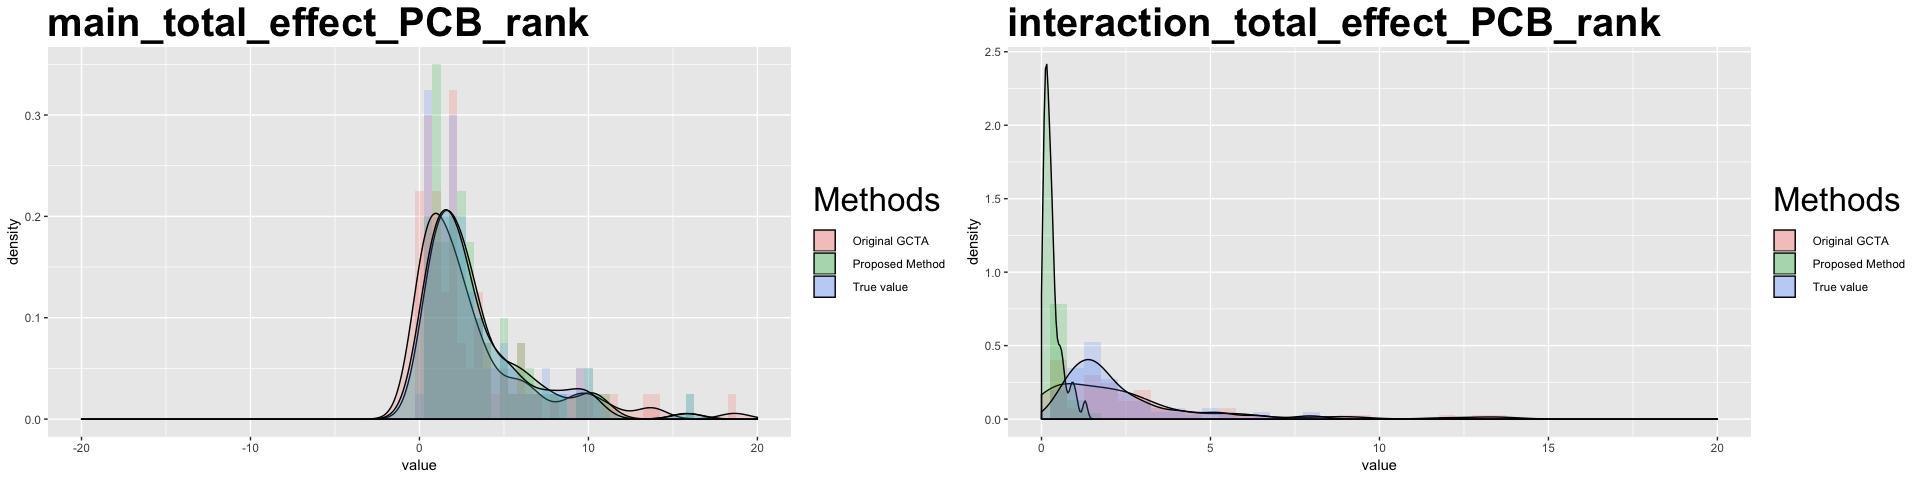
\includegraphics{./Categorize_simulation_files/figure-html/unnamed-chunk-6-1.png}

\newpage

\subsubsection{Subset}\label{subset}

To further improve the normality, I just remove several covariates which
have a very un-symmetric empirical pdf (even after normal
transformation). Therefore, after this step, most of the covariates
should have a nice symmteric bell-shape distribution.

\paragraph{simulation result}\label{simulation-result-1}

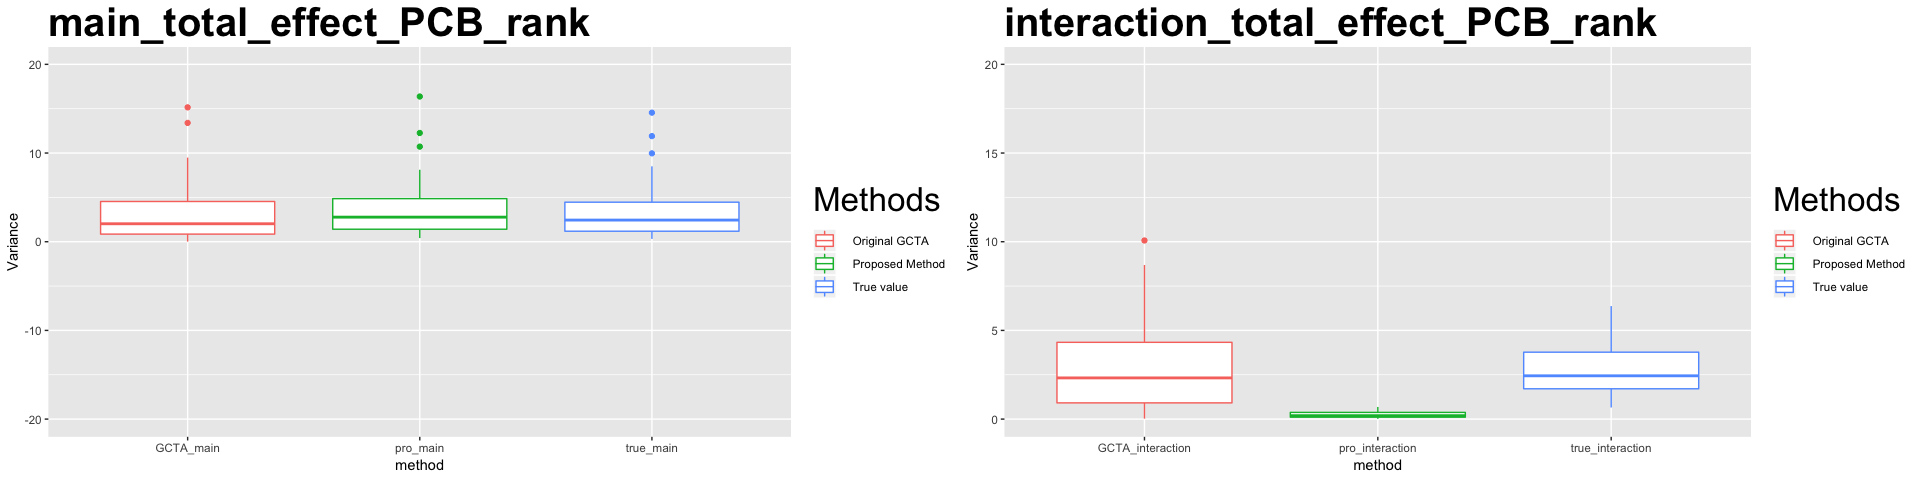
\includegraphics{./Subsetting_simulation_files/figure-html/unnamed-chunk-2-1.png}
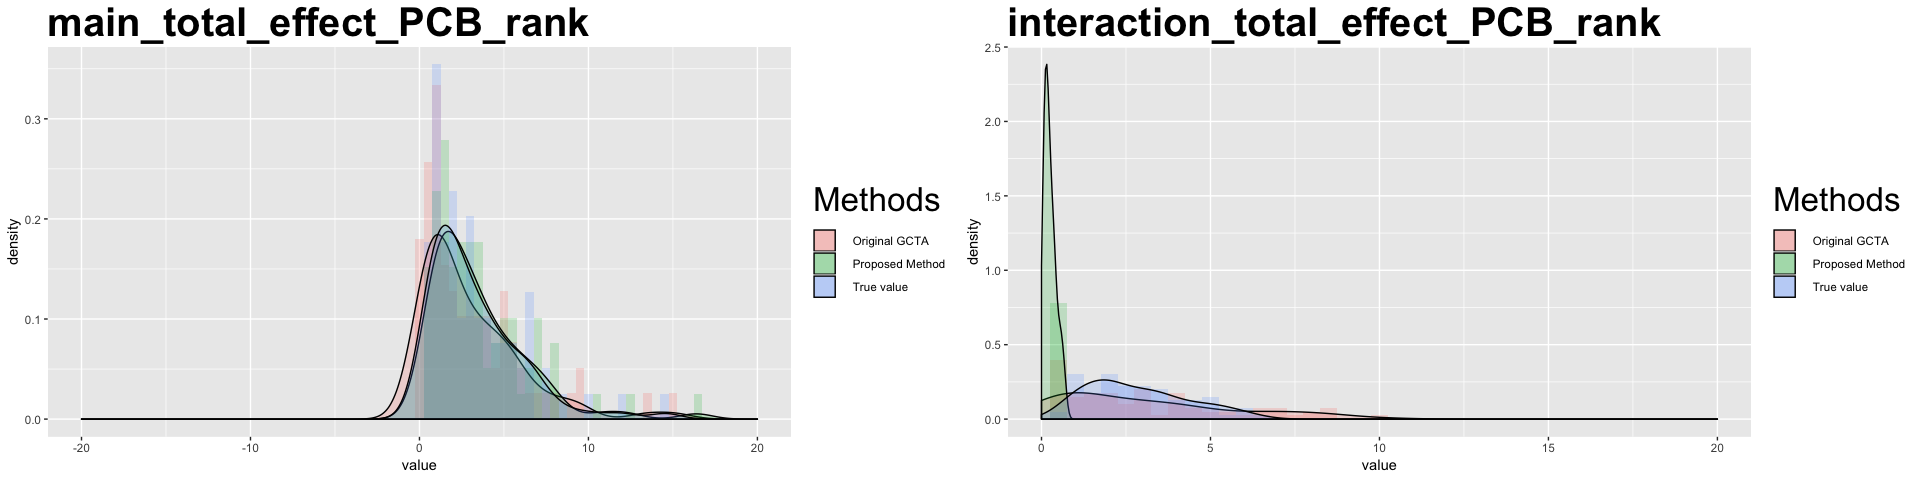
\includegraphics{./Subsetting_simulation_files/figure-html/unnamed-chunk-3-1.png}

\subsection{Questions}\label{questions}

\begin{enumerate}
\def\labelenumi{\arabic{enumi}.}
\tightlist
\item
  Since we consider the interaction terms, the covariates cannot be
  independent any more
\item
  Interaction terms are also not standardized, which means that the
  \(E(x^{(inter)}) \neq 0\)
\item
  What's will be the sparsity of the interaction terms?
\end{enumerate}

\section{Further work}\label{further-work}


\end{document}
